\documentclass[12pt, onecolumn, conference]{IEEEtran}

\usepackage{cite}
\usepackage{amsmath,amssymb,amsfonts}
\usepackage{algorithmic}
\usepackage{graphicx}
\usepackage{textcomp}
\usepackage{xcolor}
\usepackage{xspace}
\usepackage{multirow}
\usepackage{subcaption}
\usepackage{tabularx}
\usepackage{booktabs}
\usepackage{hyperref}
\hypersetup{
	colorlinks=true,
	linkcolor=blue,
	filecolor=magenta,      
	urlcolor=black,
	citecolor=black
}
\usepackage{wrapfig}



\makeatletter
\def\endthebibliography{%
	\def\@noitemerr{\@latex@warning{Empty `thebibliography' environment}}%
	\endlist
}
\makeatother

\begin{document}
	
	\title{System Description: rough draft}
	
	\author{\IEEEauthorblockN{Mia Mohammad Imran}
		\IEEEauthorblockA{\textit{Virginia Commonwealth University}\\
			Richmond, Virginia, U.S.A. \\
			imranm3@vcu.edu}
	}
	
	\maketitle
	
	\begin{abstract}

Social media posts have become an enormous source of population health. Users often share their experiences about medication intake and their effects. A fundamental step toward incorporating social media data in pharmacoepidemiologic research is to automatic medication names detection in these posts. However, detecting drug name mentioning posts are challenging as they are often informal and noisy. Medication names are often misspelled and abbreviated. The purpose of this study is to detect medication name spans in tweets.

\end{abstract}
	
	\section{Introduction}

Social media posts are often useful to detect real-time adverse drug reactions (ADR) compared to other available resources such as clinical reports, health records. They can be a valuable tool for pharmaceutical companies to obtain feedback about medication~\cite{plachouras2016quantifying, huynh2016adverse}. Vast number of tweets mentioned in drug names and adverse drug re-actions can easily be collected in real-time. Plachouras et al.~\cite{plachouras2016quantifying} reported that from July 9 to September 4, 2014 (shown in figure~\ref{fig:daily-tweets-adr}), on average 179K tweets were mentioning drug names and 721 tweets were containing ADRs. They proposed an ecosystem on clinical reports and social media posts can be useful to pharmaceutical companies - shown in figure~\ref{fig:ecosystem-pharmaceutical}.

\begin{figure}[h]
	\centering
	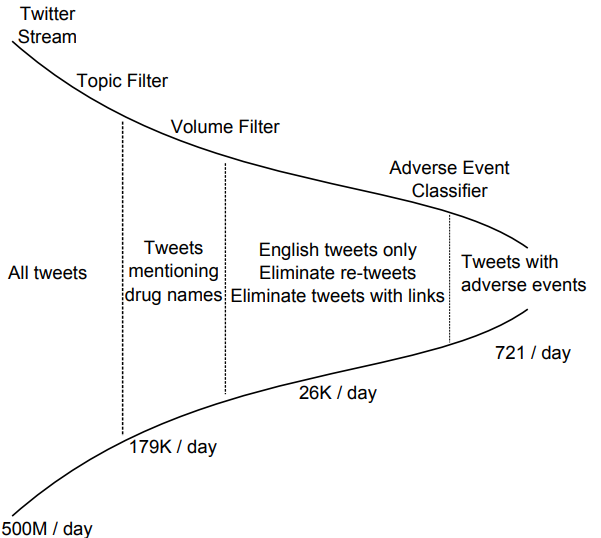
\includegraphics[width=0.99\linewidth]{Figures/g.png}
	\caption{Avg. daily tweets containing ADR from July 9 to September 4, 2014 by Plachouras et al.~\cite{plachouras2016quantifying}}
	\label{fig:daily-tweets-adr}
\end{figure}

\begin{figure}[h]
	\centering
	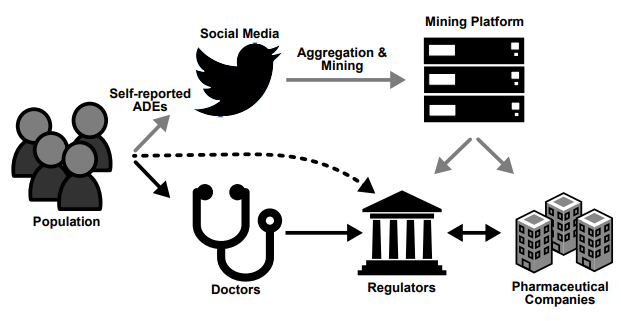
\includegraphics[width=0.99\linewidth]{Figures/j.png}
	\caption{The ecosystem of pharmaceutical companies, regulators, doctors, patients and social media Plachouras et al.~\cite{plachouras2016quantifying}.}
	\label{fig:ecosystem-pharmaceutical}
\end{figure}

The problem of detecting drug names and adverse drug reactions mentioning social media are often interrelated, both studies are often conducted simultaneously. Weissenbacher et al.~\cite{weissenbacher2018overview} noted that this research has been conducted extensively in recent years. Denecke et al.~\cite{DENECKE20091870} performed a content analysis of medical social media data, in particular question \& answer portals, weblogs, reviews, and wikis. De Rosa et al.~\cite{de114pharmacovigilance} researched on cross-relating social media contents with trusted sources such as PubMed. The researchers have essentially framed the task of medication name extraction and ADR detection as a binary classification problem. Machine learning techniques are widely used in this task. Deep learning techniques are becoming popular of late. In this paper, we will give short reviews of techniques used by various researchers. 

The review is divided into a couple of sections: preprocessing, model, annotation, evaluation.
	
	\section{Model}

\subsection{Social Media}

\subsubsection{Machine Learning}

Alvaro et al.~\cite{alvaro2015crowdsourcing} explored whether tweets contains information about first-hand medication user experience. The structure of their model is elucidated in figure~\ref{fig:flowchart-alvaro}. They used a couple of algorithms - C50, SVM, NB, Multi-Layer Perceptron (MLP), Generalized Linear Model (GLM), and Bayesian Generalized Linear Model (BGLM). In their experiment, BGLM achieved highest F1-score for almost all sets of features.

\begin{figure}[h]
	\centering
	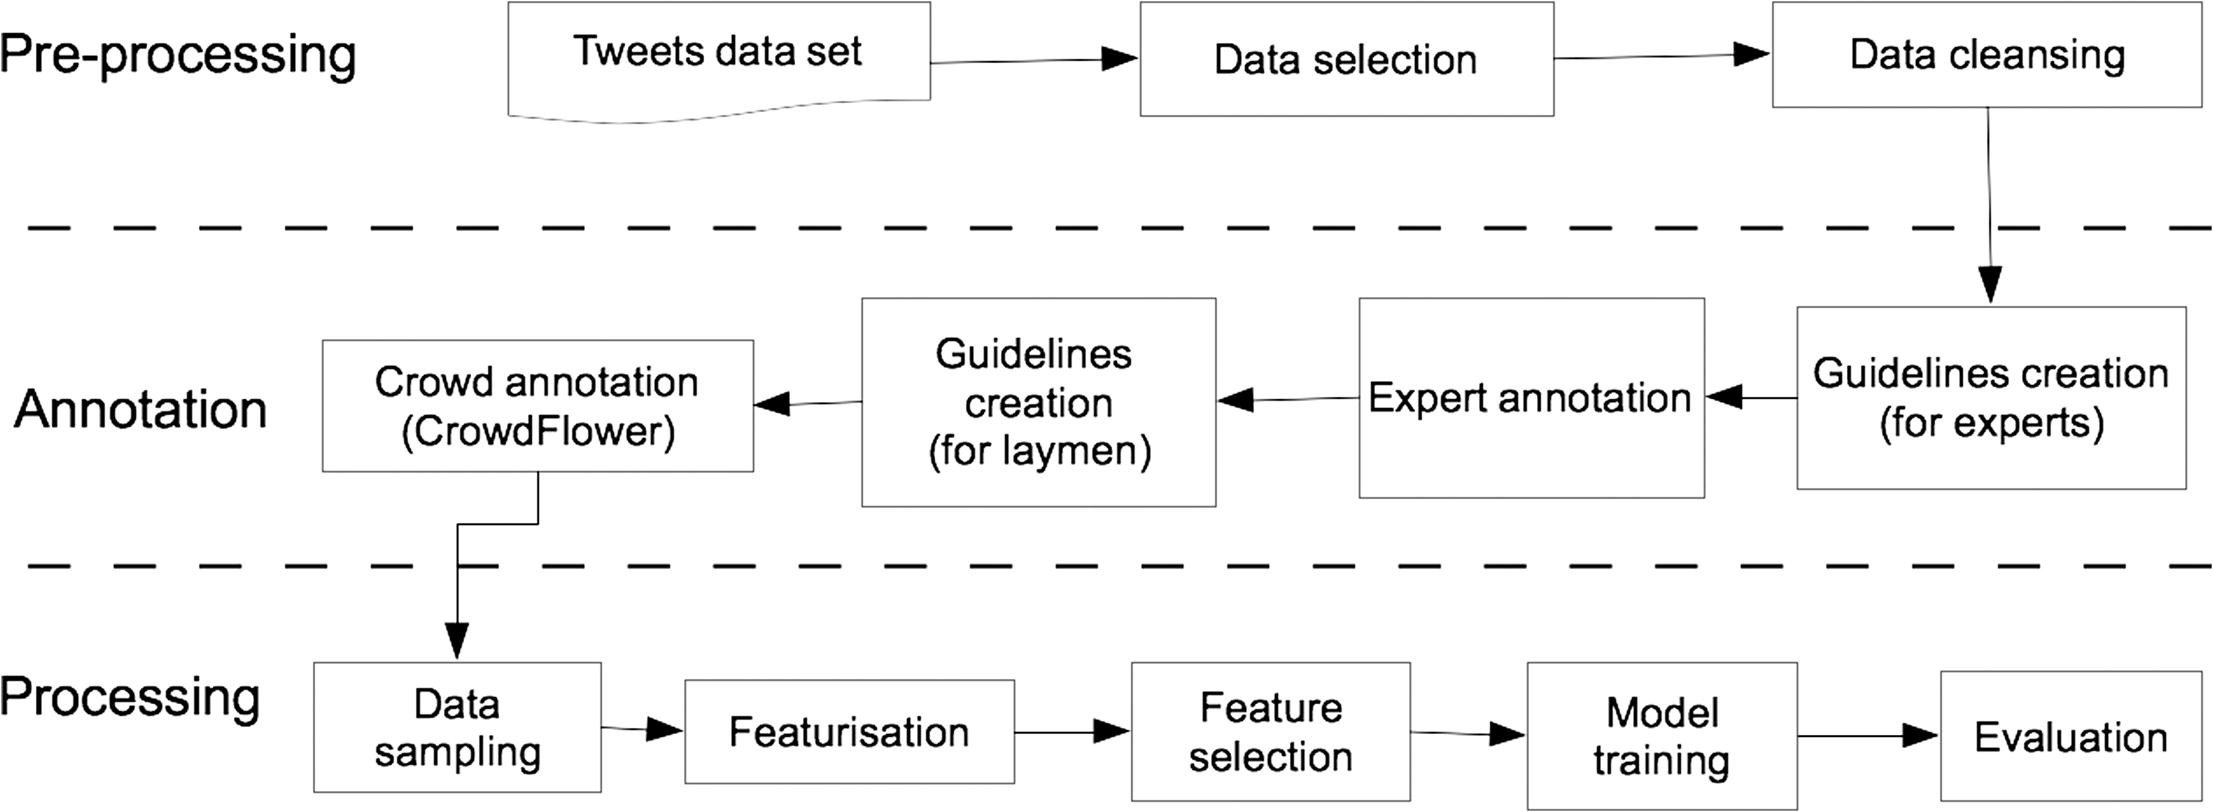
\includegraphics[width=0.99\linewidth]{Figures/n.jpg}
	\caption{Flow chart of Alvaro et al.~\cite{alvaro2015crowdsourcing}’s methodology.}
	\label{fig:flowchart-alvaro}
\end{figure}

Sarker et al.~\cite{sarker2016social} proposed a stacking based ensemble classifier to automatically detect whether tweets are abuse or not when they contain specific 4 medication names. The architecture of the methodology is shown in figure~\ref{fig:model-sarker}. In the ensemble classifier, they used four algorithms - naive bayes (NB), SVM, maximum entropy (ME), and J48, and used various features such as n-gram, abuse-indicating terms, lexicon matches, synonym expansion, word cloud. They concluded that tweets are often ambiguous and impersonal, and a large number of corpus needed for better results. A sample of their annotated data is available~\footnote{\url{http://diego.asu.edu/Publications/DrugAbuse_DrugSafety.html}}. 

\begin{figure}[h]
	\centering
	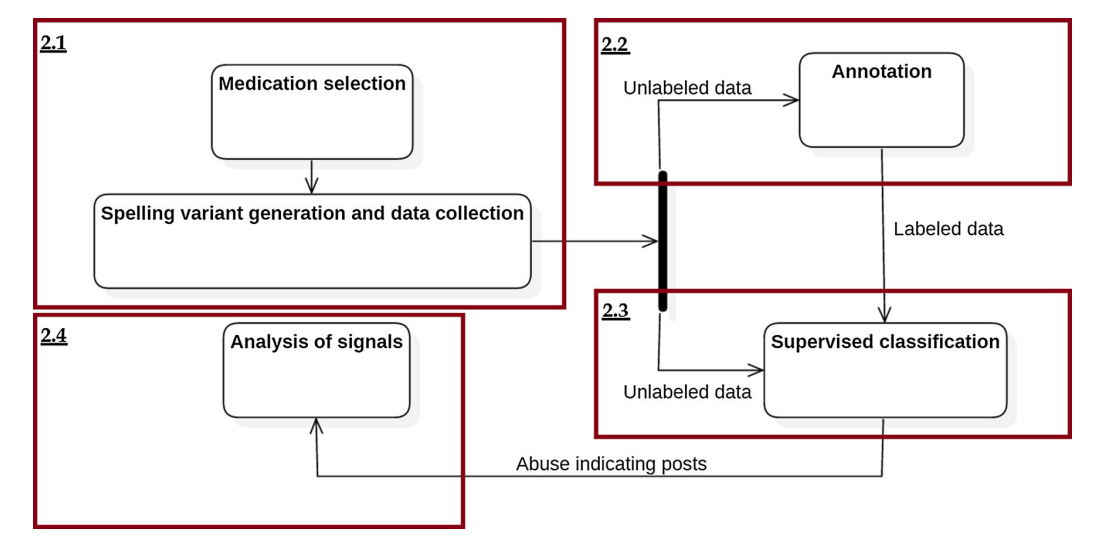
\includegraphics[width=0.99\linewidth]{Figures/h.png}
	\caption{Architecture by Sarker et al.~\cite{sarker2016social}}
	\label{fig:model-sarker}
\end{figure}

Meanwhile, to detect a tweet contains ADR or not, Zhang et al.~\cite{zhang2016ensemble} applied an ensemble algorithm of four classifiers: (1) a concept-matching classifier based on ADR lexicon; (2) a ME classifier with word-level n-gram features and TFIDF weighting scheme; (3) a ME classifier based on word-level n-grams using NB log count ratios as feature values; and (4) a ME classifier with word embedding features. They obtain an F1-score of 0.4182 (positive class). The code of their model is available~\footnote{\url{https://github.com/tjflexic/psb-adr}}.

\subsubsection{Deep Learning}

However, these approaches~\cite{sarker2016social, alvaro2015crowdsourcing, zhang2016ensemble} heavily rely on feature engineering and require large amount of expert knowledge. Recently the focus has shifted towards deep learning. Tutubalina et al.~\cite{TUTUBALINA201893} proposed a model based on bidirectional RNN for MCN in social media. The architecture is illustrated in figure~\ref{fig:architecture-tutubalina}.

\begin{figure}[h]
	\centering
	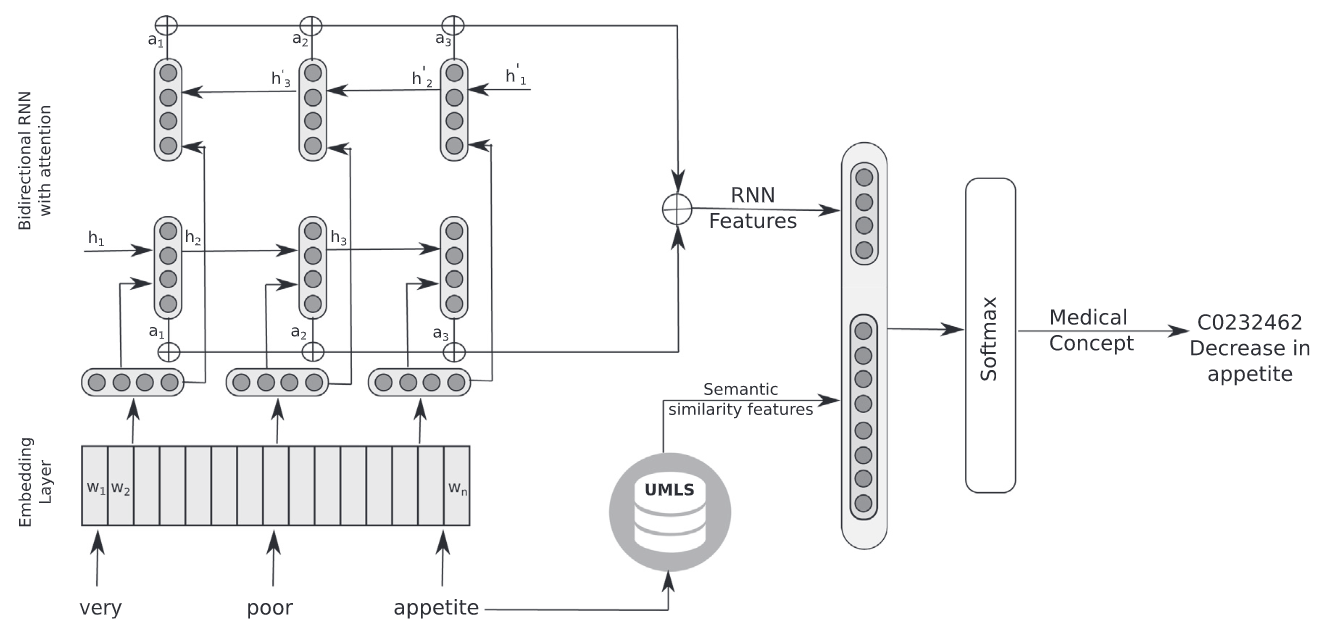
\includegraphics[width=0.99\linewidth]{Figures/f.png}
	\caption{Architecture for MCN in social media by Tutubalina et al.~\cite{TUTUBALINA201893}.}
	\label{fig:architecture-tutubalina}
\end{figure}

Huynh et al.~\cite{huynh2016adverse} investigated different neural network (NN) architecture for ADR classification. In particular, they applied their data over four algorithms: CNN, Recurrent Convolutional Neural Network (RCNN), Convolutional Recurrent Neural Network (CRNN), Convolutional Neural Network with Attention (CNNA). The architecture of these algorithms are shown in the figure 7. They compare model against Zhang et al.~\cite{zhang2016ensemble}’s model and found that CNN obtain highest F1-score. The source code of the project is available~\footnote{\url{https://github.com/trunghlt/AdverseDrugReaction}}.

\begin{figure}[h]
	\centering
	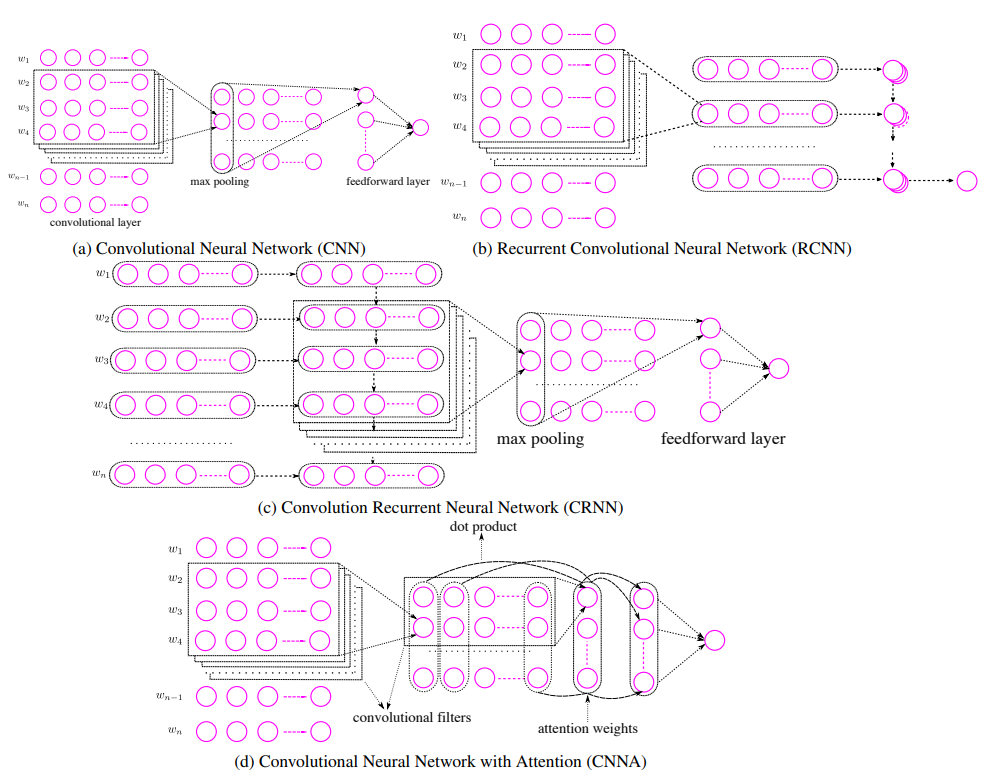
\includegraphics[width=0.99\linewidth]{Figures/e.png}
	\caption{Architecture by Huynh et al.~\cite{huynh2016adverse}.}
	\label{fig:architecture-huynh}
\end{figure}

Lee et al.~\cite{lee2017adverse}, meanwhile, applied a semi-supervised CNN framework for the same task. This model was developed by Johnson et al.~\cite{johnson2015semi}. Lee et al. found that this model outperform a strong state-of-the-art supervised classification model by +9.9\% F1-score. The architecture of the model is shown in the figure~\ref{fig:architecture-lee}. The method works in two phases: (1) unsupervised phrase embedding learning, and (2) integrating the learned embeddings into the supervised training that uses labeled data.

\begin{figure}[h]
	\centering
	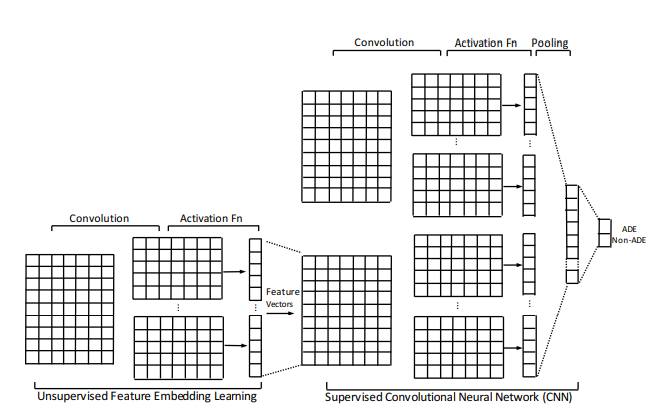
\includegraphics[width=0.99\linewidth]{Figures/l.png}
	\caption{Semi-supervised CNN by Lee et al.~\cite{lee2017adverse}.}
	\label{fig:architecture-lee}
\end{figure}

Weissenbacher et al.~\cite{weissenbacher2019deep} introduced a deep neural networks ensemble method - \textit{Kusuri} - a LSTM model - to detect medication names in unbalanced tweets. \textit{Kusuri} is composed of two modules: first, applied four different classifiers (lexicon based, spelling variant based, pattern based, and a weakly trained neural network) parallel to discover potential tweets with medication names; second, an ensemble of deep neural networks encoding morphological, semantic, and longrange dependencies of important words in the tweets makes the final decision. The architecture is shown in figure~\ref{fig:architecture-weissenbacher}. This model achieves an F1-score of 0.788 on an extremely unbalanced dataset (98959 tweets, with only 0.26\% mentioning medications). A brief description of four algorithms are provided by the authors~\footnote{\url{https://tinyurl.com/y47qzbcq}}.

\begin{figure}[h]
	\centering
	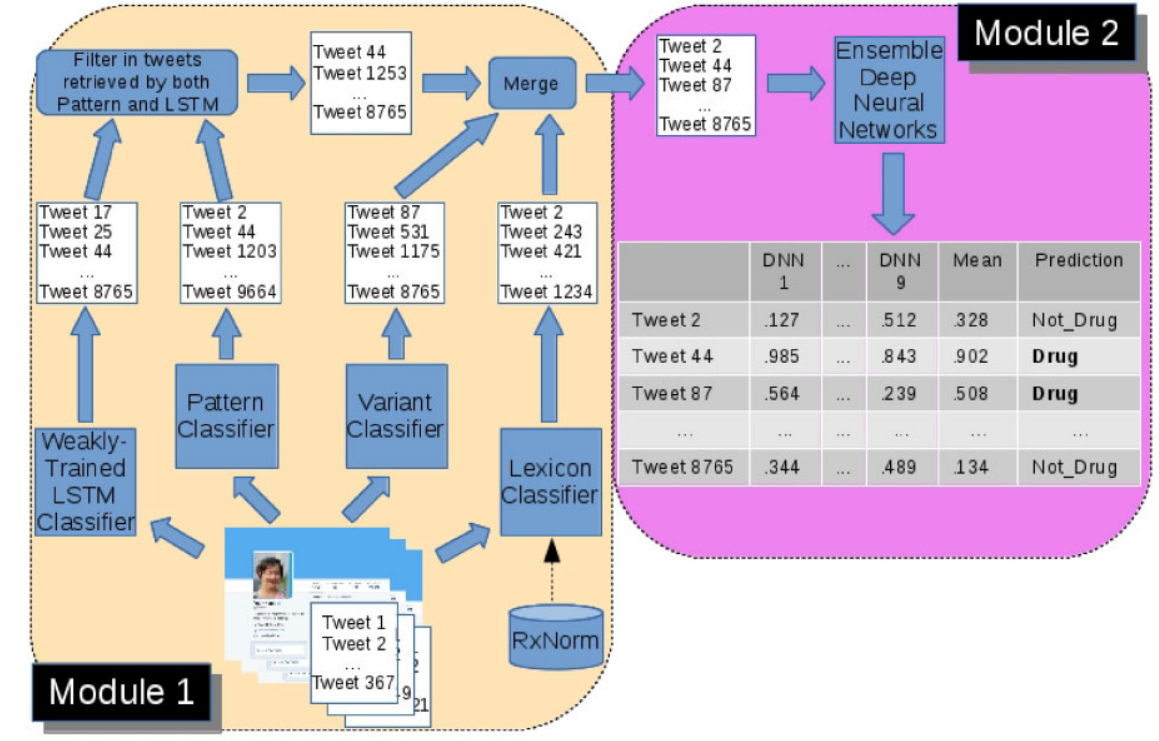
\includegraphics[width=0.99\linewidth]{Figures/a.png}
	\caption{\textit{Kusuri} model by Weissenbacher et al.~\cite{weissenbacher2019deep}.}
	\label{fig:architecture-weissenbacher}
\end{figure}

Wu et al.~\cite{wu2019msa} proposed neural approach using multi-head self-attention (MSA) to jointly detect drug name and adverse drug reaction. Their MSA model has three modules: first, a word representation module, which aims to build the contextual representations of words from the original characters within them; second, a tweet representation module; third, a classification module. The framework of the model is illustrated in the figure~\ref{fig:architecture-wu-msa}.

\begin{figure}[h]
	\centering
	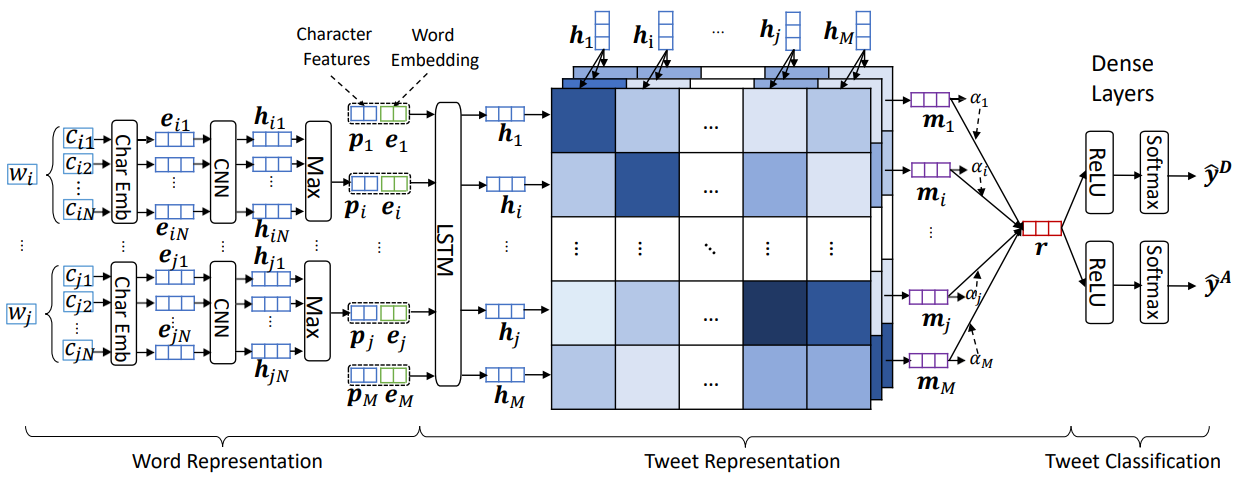
\includegraphics[width=0.99\linewidth]{Figures/k.png}
	\caption{MSA model by Wu et al.~\cite{wu2019msa}.}
	\label{fig:architecture-wu-msa} 
\end{figure}

\subsection{Clinical Texts and Health Records}

Researches has been conducted thoroughly to extract medication names from clinical texts and health records~\cite{weeks2020medextractr, kim2020ensemble, ju2020ensemble}. 2018 n2c2 shared task on adverse drug events and medication extraction~\footnote{\url{https://portal.dbmi.hms.harvard.edu/projects/n2c2-2018-t2/}}, Kim et al.~\cite{kim2020ensemble} demonstrated that a stacked ensemble with a search-based structured prediction algorithm achieved good performance (an F1 score of 0.9266 on official dataset) by effectively integrating the output of individual classifiers. Their architecture is shown in figure~\ref{fig:architecture-kim}.

\begin{figure}[h]
	\centering
	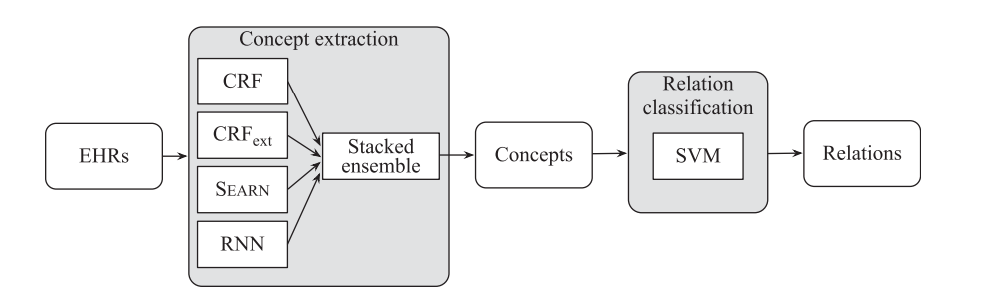
\includegraphics[width=0.99\linewidth]{Figures/i.png}
	\caption{Framework of model by Kim et al.~\cite{kim2020ensemble}.}
	\label{fig:architecture-kim}
\end{figure}

Ju et al.~\cite{ju2020ensemble} proposed an ensembling system based on neural network to automatically extract adverse drug events and drug related entities from clinical narratives. They firstly pre-processed Electronic Health Records(EHR) using sentence segmentation and tokenization. Then they implemented feature based and neural network-based models to detect ADEs and related medications. The architecture is shown in figure~\ref{fig:architecture-ju}. Their method achieved 92.78\% lenient micro F1-score, with 95.99\% lenient precision, and 89.79\% lenient recall.

\begin{figure}[h]
	\centering
	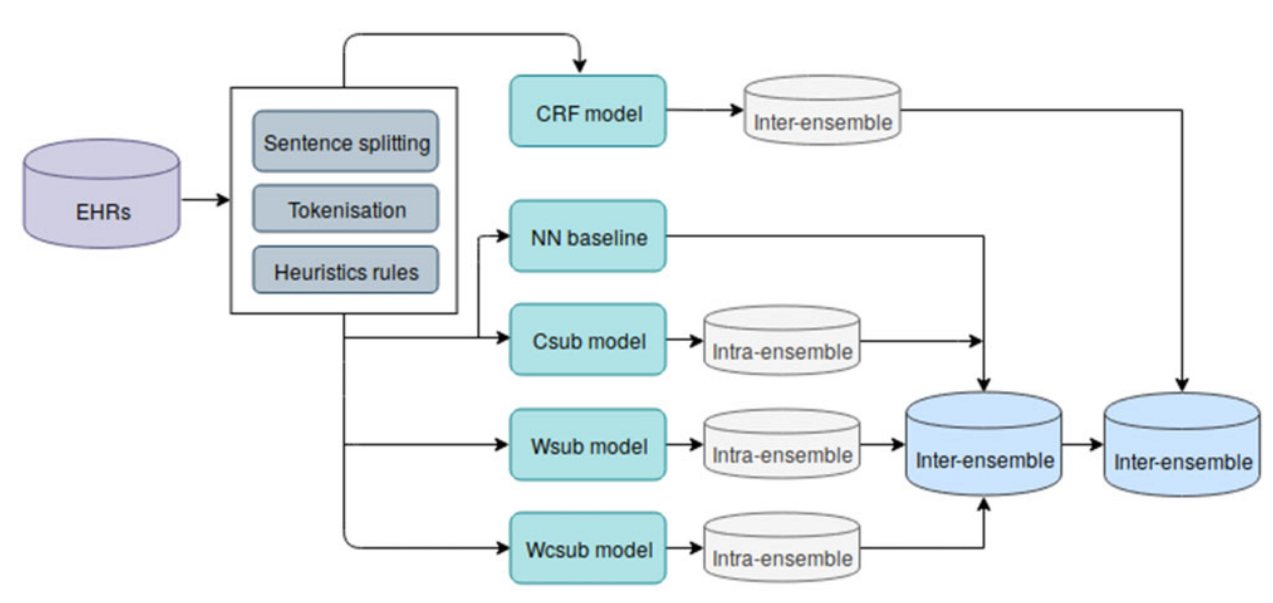
\includegraphics[width=0.99\linewidth]{Figures/c.png}
	\caption{Framework of model by Ju et al.~\cite{ju2020ensemble}.}
	\label{fig:architecture-ju}
\end{figure}

The research of extracting medication names in other languages has been an area of interest as well. Armengol-Estape et al.~\cite{armengol2019pharmaconer} proposed a deep learning-based tool for automatically finding chemicals and drugs in Spanish medical texts.

	\section{Evaluation}

Over the years, different techniques have been applied for preprocessing, model development, and annotation. Machine learning approaches have been widely used. Deep learning techniques are gradually replacing them and becoming more successful to detect medication names and ADR events.

For ADR classification, among the machine learning-based models, Jonnagaddala et al.~\cite{jonnagaddala2016binary}, in their binary classification, managed to achieve an F-score of 0.33. Meanwhile, Zhang et al.~\cite{zhang2016ensemble}'s ensemble method obtained an F-score of 0.4182 and Sarker et al.~\cite{sarker2016social}'s ensemble method obtained an F-score of 0.46.  Huynh et al.~\cite{huynh2016adverse} compared their deep learning-based model against Zhang et al.~\cite{zhang2016ensemble}’s model. On twitter dataset, their~\cite{huynh2016adverse} model achieved an F-score of 0.51, 0.51, 0.49, and 0.49 using CNN, CRNN, RCNN, and CNNA respectively compared to baseline model's 0.40 F-score. On an unbalanced dataset, Lee et al.~\cite{lee2017adverse}'s Semi-Supervised CNN model for ADR classification outperforms the state-of-the-art supervised ADR classifier from previous work~\cite{sarker2015portable} by +9.9\%. Wu et al.~\cite{wu2019msa} compared their MSA model with Lee et al.~\cite{lee2017adverse}. On a twitter dataset, where Lee et al.'~\cite{lee2017adverse}s model achieved an F-score of 0.503, Wu et al.~\cite{wu2019msa} managed to obtain 0.524. However, Alimova et al.~\cite{alimova2017automated} showed that it's possible to achieve better results using machine learching techniques compared to neural networks when the model is feature-rich. On a twitter dataset, their model~\cite{alimova2017automated} achieved an F-score of 0.702 using SVM and 0.737 using LR against a CNN baseline which achieved 0.702.

Meanwhile, on the research of detecting medication names, Jimeno-Yepes et al.~\cite{jimeno2015identifying} achieved an F-score of 0.65 on a corpus of 1300 tweets using a method based on conditional random fields. Wu et a.~\cite{wu2018detecting} achieved an F-score of 0.9183 using their MSA model on a balanced dataset. Weissenbacher et al.~\cite{weissenbacher2019deep} obtained an F-score of 0.788 on an extremely unbalanced dataset (98959 tweets, with only 0.26\% mentioning medications) and 0.937 on a balanced dataset(50-50 corpus of 15005 tweets) using deep learning methodologies.
		
	\section{Limitations and Future Work}
	One of key area, we can improve in our dataset, is preprocessing the hashtags. Usually, the hashtags are combinations of multiple words. But we had not considered this when preprocessing out data. Another major drawback of our system is recognizing medication and dietary names. We have used pre-compiled medications list. The other issue, we had faced, the model was predicting correctly that there's a medication name but the medication terms are abstract - like `birth control pill', `meds', etc. 
	
	Our future work will involve performance over extremely balanced dataset where positive classes are 0.2-0.3\%. And secondly, we will work on to improve the methodology on how to detect medication and dietary names. As the dataset is highly imbalanced, especially, when there are 0.3\% positive classes, performance can be improved by upsampling minority class, by downsampling majority class, and adding weight when sampling~\footnote{\url{https://www.tensorflow.org/tutorials/structured_data/imbalanced_data}}. Secondly,	We can improve the detection of the medication names by using name-entity recognition (NER).
	
	\section{Conclusion}
	In this paper, we have presented a model of learning classifier to identify tweets mentioning medication names. The model was able to achieve an f1-score of 0.94 on an imbalanced dataset with 1.88\% positive class. However, it achieved less success for even more imbalanced dataset with 0.38\% positive class. The code, dataset, and the model used for these experiments are publicly available~\footnote{\url{https://github.com/imranraad07/cmsc-516/tree/main/my_project}}.

	\section{Acknowledgment}
	The authors acknowledge the help of Mr. Davy Weissenbacher for kindly sharing the dataset.

	\bibliographystyle{IEEEtran}
	\bibliography{paper}
	
\end{document}